\documentclass[letterpaper,12pt,oneside]{article}

% --- Package Config ---
\usepackage[utf8]{inputenc}         % Character encoding
\usepackage[spanish]{babel}         % Spanish language support
\usepackage{csquotes}               % Recommended by biblatex for babel compatibility
\usepackage{lmodern}                % Latin Modern font
\usepackage[T1]{fontenc}            % Codificación de salida de caracteres (obligatorio para copiar bien)

% Page Layout and Margins
\usepackage{ragged2e}               % Justify text
\usepackage{anysize}                % Flexible margin settings

% \marginsize{3cm}{2.5cm}{1cm}{2cm} % Example: {left}{right}{top}{bottom}

% Tables
\usepackage{float}                  % Improved table/figure placement
\usepackage{booktabs}               % Professional-quality tables
\usepackage{tabularx}               % Tables with flexible width
\usepackage{longtable}              % Tables spanning multiple pages
\usepackage{array}                  % Extended column definitions
\usepackage{pbox}                   % Line breaks in table cells
\usepackage{colortbl}               % Color in tables

% Math
\usepackage{amsmath}                % Advanced math typesetting

% Graphics and Rotation
\usepackage{rotating}               % Rotate tables and figures
\usepackage{pdflscape}              % Landscape pages in PDF

% Colors
\usepackage{color}                  % Colored text
\definecolor{naranja}{rgb}{1,0.5,0}
\definecolor{rojo}{rgb}{1,0,0}
\definecolor{SteelBlue}{rgb}{0.3,0.5,0.7}

% Hyperlinks
\usepackage[pdftex,unicode,bookmarks=true,linkcolor=black,citecolor=black,colorlinks=true,urlcolor=black]{hyperref}

% Figures and Sub figures
\usepackage{subfig}                 % Sub figures
\usepackage{enumitem}               % Customizable lists
\usepackage{url}                    % URL formatting
\usepackage{caption}
\usepackage{adjustbox}
\captionsetup{skip=1em, font=small}
\captionsetup[table]{name=Tabla}

% Bibliography
\usepackage[style=ieee]{biblatex}   % IEEE bibliography style
\usepackage[numbib,notlof,notlot,nottoc]{tocbibind} % Numbered bibliography in ToC
\addbibresource{bibliografia.bib}

% Tables
\renewcommand\arraystretch{1.4}
\captionsetup[table]{justification=centering}

% Renaming for Spanish
\addto\captionsspanish{
  \renewcommand{\contentsname}{Tabla de Contenido}
}
\addto\captionsspanish{
  \renewcommand{\listtablename}{Índice de Tablas}
}
\addto\captionsspanish{
  \renewcommand{\listfigurename}{Índice de Figuras}
}

% Custom Spaces between paragraphs
\setlength{\parskip}{1em}
\setlength{\parindent}{0pt}

% ---------- Document Setup ----------
\begin{document}
\justifying % Justify text in the document
\newcommand{\grayTableHeaderCell}[2]{%
  \multicolumn{1}{|c|}{\cellcolor[gray]{0.9}%
    \parbox[c]{#1}{\centering\textbf{#2}}
  }
}

\newcommand{\tableCell}[1]{
  \vspace{4pt} % más aire arriba
  #1
  \vspace{4pt} % más aire abajo
}
 % Include utility commands

% avoid magic strings with objetivos específicos
\newcommand\objetivoEspecificoA{Reescribir la lógica crítica de la aplicación actualmente implementada en el cliente, para ser ejecutada de forma segura en AWS Lambda.}

\newcommand\objetivoEspecificoB{Actualizar progresivamente la base de código de la aplicación \textit{backend} y \textit{frontend} para reemplazar las dependencias actuales de Firebase por servicios equivalentes de AWS.}

\newcommand\objetivoEspecificoC{Diseñar e implementar una arquitectura centralizada en AWS que facilite la migración de la base de datos y de los registros de usuarios desde Firebase, incluyendo la construcción de una pipeline ETL basada en servicios como Step Functions, Lambda y SQS.}

\newcommand\objetivoEspecificoD{Implementar pruebas automatizadas sobre el código refactorizado durante la migración, así como una pipeline de integración continua (CI).}

% Activities
% - Objective A
\newcommand{\objectivoEspecificoAActividadadA}{
  Identificación de lógica crítica actual en el \textit{frontend}.
}
\newcommand{\objectivoEspecificoAActividadadB}{
  Diseño de funciones Lambda seguras.
}
\newcommand{\objectivoEspecificoAActividadadC}{
  Implementación y pruebas de funciones.
}
\newcommand{\objectivoEspecificoAActividadadD}{
  Despliegue en entorno AWS.
}

% - Objective B
\newcommand{\objectivoEspecificoBActividadadA}{
  Identificación de dependencias actuales a Firebase.
}
\newcommand{\objectivoEspecificoBActividadadB}{
  Selección de servicios AWS equivalentes.
}
\newcommand{\objectivoEspecificoBActividadadC}{
  Refactorización e integración.
}
\newcommand{\objectivoEspecificoBActividadadD}{
  Validación de funcionamiento.
}

% - Objective C
\newcommand{\objectivoEspecificoCActividadadA}{
  Levantamiento de arquitectura actual.
}
\newcommand{\objectivoEspecificoCActividadadB}{
  Diseño de nueva arquitectura AWS.
}
\newcommand{\objectivoEspecificoCActividadadC}{
  Implementación de migración de datos y usuarios.
}
\newcommand{\objectivoEspecificoCActividadadD}{
  Validación y pruebas.
}

% - Objective D
\newcommand{\objectivoEspecificoDActividadadA}{
  Identificación de componentes críticos a testear.
}
\newcommand{\objectivoEspecificoDActividadadB}{
  Desarrollo de pruebas automatizadas
}
\newcommand{\objectivoEspecificoDActividadadC}{
  Implementación de pipeline de CI.
}
\newcommand{\objectivoEspecificoDActividadadD}{
  Validación continua.
}

% - Objective Document
\newcommand{\objetivoEspecificoDocumentActividadA}{
  Redacción progresiva.
}
\newcommand{\objetivoEspecificoDocumentActividadB}{
  Revisión con tutor.
}
\newcommand{\objetivoEspecificoDocumentActividadC}{
  Preparación para entrega y defensa.
}

\newcommand{\objetivoEspecificoAActividades}{
  \begin{enumerate}[leftmargin=*, topsep=0pt, itemsep=0pt]
    \item \objectivoEspecificoAActividadadA
    \item \objectivoEspecificoAActividadadB
    \item \objectivoEspecificoAActividadadC
    \item \objectivoEspecificoAActividadadD
  \end{enumerate}
}

\newcommand{\objetivoEspecificoBActividades}{
  \begin{enumerate}[leftmargin=*, topsep=0pt, itemsep=0pt]
    \item \objectivoEspecificoBActividadadA
    \item \objectivoEspecificoBActividadadB
    \item \objectivoEspecificoBActividadadC
    \item \objectivoEspecificoBActividadadD
  \end{enumerate}
}

\newcommand{\objetivoEspecificoCActividades}{
  \begin{enumerate}[leftmargin=*, topsep=0pt, itemsep=0pt]
    \item \objectivoEspecificoCActividadadA
    \item \objectivoEspecificoCActividadadB
    \item \objectivoEspecificoCActividadadC
    \item \objectivoEspecificoCActividadadD
  \end{enumerate}
}
\newcommand{\objetivoEspecificoDActividades}{
  \begin{enumerate}[leftmargin=*, topsep=0pt, itemsep=0pt]
    \item \objectivoEspecificoDActividadadA
    \item \objectivoEspecificoDActividadadB
    \item \objectivoEspecificoDActividadadC
    \item \objectivoEspecificoDActividadadD
  \end{enumerate}
}

\newcommand{\objetivoEspecificoDocumentActividades}{
  \begin{enumerate}[leftmargin=*, topsep=0pt, itemsep=0pt]
    \item \objetivoEspecificoDocumentActividadA
    \item \objetivoEspecificoDocumentActividadB
    \item \objetivoEspecificoDocumentActividadC
  \end{enumerate}
}
 %  variables for specific objectives

% -- Portada, Contraportada y Resumen --
% Avoid magic strings
\newcommand{\titulo}{Migración de la infraestructura de Firebase a AWS en Paralegales}
\newcommand{\subtitulo}{Pasantía en Modalidad de Convenio}
\newcommand{\autor}{Juan Felipe Monsalve Vargas}
\newcommand{\correoDirector}{royer.estrada@correounivalle.edu.co}
\newcommand{\universidad}{Universidad del Valle}
\newcommand{\facultad}{Facultad de Ingeniería}
\newcommand{\escuela}{Escuela de Ingeniería de Sistemas y Computación}
\newcommand{\sede}{Sede (06) Tuluá}
\newcommand{\anio}{2025}

\newcommand\portada{
  \begin{titlepage}
    \begin{center}
      \begin{figure}[h]
        \centering
        
\includegraphics[width=0.1\textwidth]{img/template/univalle-escudo.jpg}
      \end{figure}
      {\bf \titulo }
      \vspace{0.5cm}
      {\bf \subtitulo }
      \vfill
      {\bf \autor }
      \vfill
      {\bf \universidad  \par}
      {\bf \facultad \par}
      {\bf \escuela \par}
      {\bf \sede \par}
      {\bf \anio \par}
    \end{center}
  \end{titlepage}
}

\newcommand\contraportada{
  \begin{titlepage}
    \begin{center}
      {\bf \titulo }
      \vspace{0.5cm}
      {\bf \subtitulo }
      \vfill
      \vfill
      \vfill
      {\bf \autor \par}
      {\bf Código 202160145 \par}
      {\url{ juan.felipe.monsalve@correounivalle.edu.co } \par}
      \vfill
      \vfill
      \vfill
      {Director \par}
      {\bf Ms.C Royer David Estrada Esponda. Ing \par}
      {Profesor de la Escuela de Ingeniería de Sistemas y Computación \par}
      {\url{royer.estrada@correounivalle.edu.co} \par}
      \vfill
      \vfill
      \vfill
      \vfill
      {\bf \universidad  \par}
      {\bf \facultad \par}
      {\bf \escuela \par}
      {\bf \sede \par}
      {\bf \anio \par}
    \end{center}
  \end{titlepage}
}
\portada
\contraportada
\newpage
\section*{Resumen}

Paralegales es una plataforma de legaltech orientada a automatizar el seguimiento de procesos judiciales en la Rama Judicial Unificada en Colombia. El objetivo principal de esta solución es simplificar la tarea de los abogados al ofrecer herramientas que permiten monitorear automáticamente los cambios en los procesos judiciales, además de proporcionar funcionalidades complementarias para mejorar la eficiencia en la gestión legal.

Para acelerar la salida a producción, el desarrollo de Paralegales se hizo uso del Software Development Kit (SDK) de Firebase, lo que permitió avanzar rápidamente en funcionalidades clave. Sin embargo, esta decisión trajo consigo importantes compromisos técnicos, como la implementación de lógica de negocio crítica directamente en el frontend, lo que representa riesgos de seguridad y dificultades para aplicar principios de escalabilidad.

El presente proyecto tiene como objetivo principal migrar y adaptar la infraestructura tecnológica de Paralegales desde Firebase hacia un entorno 100\% en AWS (Amazon Web Services). Esta migración busca mejorar la seguridad del sistema, aumentar la escalabilidad y reducir los costos operativos, además de permitir trasladar lógica de negocio sensible actualmente implementada en el frontend hacia entornos seguros como AWS Lambda.

\hfill

\textbf{Palabras clave:}  Ingeniería de software, Microservicios, Enterprise migration, Cloud computing, APIs, Vendor lock-in, Legaltech.


% -- Indices --
\tableofcontents

\newpage
\listoftables

\newpage
\listoffigures

% -- Chapters --
\section{Introducción}

En Colombia, el acceso a la información judicial se ha centralizado mediante el Portal  “Rama Judicial Unificada”, una página web donde cualquier ciudadano puede consultar el estado de los procesos legales. Sin embargo, este sistema no cuenta con mecanismos automatizados de seguimiento o notificación de cambios, lo cual obliga a los profesionales del derecho a revisar constantemente el estado de cada proceso de forma manual \cite{Paez2024}. Sumado a esto,  según el Consejo Superior de la Judicatura para el 2023 el índice de congestión de la justicia en Colombia fue de 54.9\% \cite{Rozo2024}. Esta situación, especialmente crítica para abogados que gestionan múltiples casos, no solo representa una carga operativa considerable, sino que también incrementa el riesgo de omitir actualizaciones importantes que pueden afectar el desarrollo de los casos.

Ante este panorama, se abre una clara oportunidad de negocio para desarrollar software que automatice y optimice esta tarea, además de ofrecer funcionalidades adicionales que permitan aprovechar este nicho de mercado. Todo esto, de la mano de tecnologías emergentes como la inteligencia artificial, la computación, entre otras. Estas tecnologías permiten no solo reducir la carga operativa del profesional jurídico, sino también mejorar la calidad del servicio prestado al cliente \cite{Botero2023}. En este contexto, el sector \textit{Legaltech} ha ganado tracción en Colombia y Latinoamérica, Siendo Colombia quien ocupa el segundo lugar en cuanto a productos de software en la industria jurídica según el Legal Tech Index \cite{Sierra2023}.

En este marco surge Paralegales, una plataforma desarrollada por la empresa Webcloster S.A.S., cuyo propósito es automatizar el seguimiento de procesos judiciales y brindar a los abogados una experiencia más eficiente, inteligente y centralizada. Este proyecto de grado tiene como objetivo migrar la infraestructura actual de Paralegales, basada parcialmente en Firebase, hacia un entorno 100\% en AWS. Esta migración permitirá mejorar la seguridad de la lógica de negocio, actualmente expuesta en el cliente (\textit{frontend}), aumentar la escalabilidad del sistema y reducir los costos operativos. Además, se buscará aplicar las mejores prácticas de ingeniería de software dentro de lo posible para fortalecer la calidad técnica del producto durante su evolución.

\section{Descripción de la empresa}

\subsection{Descripción General}
Webcloster S.A.S. es una empresa del sector de tecnologías de la información y la comunicación que, en respuesta a las necesidades del entorno, innova en la forma de trabajar y administrar recursos mediante la creación de plataformas tecnológicas de servicios. A través de sus propios sistemas de información, la compañía apoya a organizaciones de todos los tamaños para que puedan alcanzar su máximo potencial mediante las soluciones tecnológicas que ofrece.

\subsection{Misión}
Empresa dedicada a la creación y desarrollo de Software que facilita la gestión y administración efectiva de las operaciones empresariales y personales, brindando soluciones innovadoras que se adaptan a las necesidades de nuestros clientes buscando siempre incrementar la productividad y competitividad con servicios de alto valor agregado, y confiabilidad.

\subsection{Visión}
Establecer un posicionamiento en el sector de las TIC; implementado los cambios que la globalización demande con respecto al desarrollo de software y aplicativos móviles, mejorando continuamente cada uno de los procesos implementados, cumpliendo requerimientos de nuestros clientes y comprometidos de forma transparente con sus necesidades.

\subsection{Valores Corporativos}
\begin{itemize}
  \item \textbf{Honestidad:}  es vital la transparencia y sinceridad.
  \item \textbf{Pasión:} "Disfrutar lo que hacemos"
  \item \textbf{Puntualidad:} Tener especial consideración con el tiempo de clientes, proveedores y jefes.
  \item \textbf{Calidad:} Garantizar los mejores productos y servicios ante el mundo.
  \item \textbf{Trabajo en equipo:} Tolerancia, respeto, admiración, lealtad y solidaridad.
  \item \textbf{Orientación al cliente:} adecuarnos a las necesidades de nuestros clientes.
  \item \textbf{Mejora Continua:} Mejora y revolución de procesos, productos y servicios para aumentar la calidad y satisfacción de resultados de forma sostenible.
  \item \textbf{Resolución de problemas:} Incentivamos el pensamiento de nuestros colaboradores orientado a la búsqueda de soluciones culpables óptimas para mejorar y no buscar
  \item \textbf{Responsabilidad Social:} Causar un impacto amplio y positivo ante la sociedad que nos rodea.
\end{itemize}

% TODO: Organigrama de Webcloster

\section{Formulación del problema}

\subsection{Descripción del problema}
Actualmente, la plataforma Paralegales presenta una serie de problemas estructurales derivados de decisiones técnicas tomadas durante su etapa inicial de desarrollo. Como se aprecia en la \autoref{fig:arbol_problemas}, el principal problema identificado es la exposición de lógica de negocio crítica en el cliente, lo que genera una serie de consecuencias negativas a nivel de seguridad, arquitectura, costos y gestión tecnológica.

Uno de los efectos más graves de esta exposición es el alto riesgo de inseguridad en la plataforma, ya que la lógica sensible puede ser inspeccionada, manipulada o replicada por terceros, lo que constituye un ejemplo de \textit{Insecure Design}, una categoría de riesgo identificada en el OWASP Top 10 \cite{OWASP2021}.

Además, la dependencia de servicios propietarios como Firebase, fenómeno conocido como \textit{vendor lock-in} \cite{OparaMartins2016, OparaMartins2014,Harauzek2022}, genera costos operativos más elevados y compromete la viabilidad económica de la plataforma a largo plazo. Asimismo, la falta de centralización en un único ecosistema tecnológico provoca fragmentación, lo que dificulta la integración, el mantenimiento y la escalabilidad del sistema.

Actualmente, Paralegales utiliza funciones AWS Lambda (\textit{backend}) para manejar algunos casos de uso que requieren lógica crítica del lado del servidor. Sin embargo, mantener lógica crítica tanto en el \textit{frontend} como en el \textit{backend} agrava la fragmentación tecnológica. Desde el punto de vista de diseño de sistemas (\textit{system design}), esta dispersión de componentes críticos genera una arquitectura inconsistente y difícil de escalar y mantener, como se ilustra también en la \autoref{fig:arbol_problemas}.

En la raíz del problema, como se expone en la \autoref{fig:arbol_problemas}, se encuentra la priorización de la velocidad en el desarrollo sobre la adopción de buenas prácticas \cite{BirrEngwall2024}. Esta decisión condujo a una dependencia parcial de Firebase y sus tecnologías propietarias, así como a la omisión de delegar lógica crítica en entornos de ejecución que corren del lado del servidor como AWS Lambda o Cloud Functions, incrementando los riesgos mencionados.

Por lo tanto, se evidencia la necesidad urgente de una reestructuración tecnológica que permita resolver estos problemas, mejorando la seguridad, reduciendo costos, y garantizando una arquitectura sólida y escalable para el futuro del proyecto.

\newcommand\captionArbolProblemas{Árbol de problemas.\hspace{1em}}

\begin{figure}[H]
  \centering
  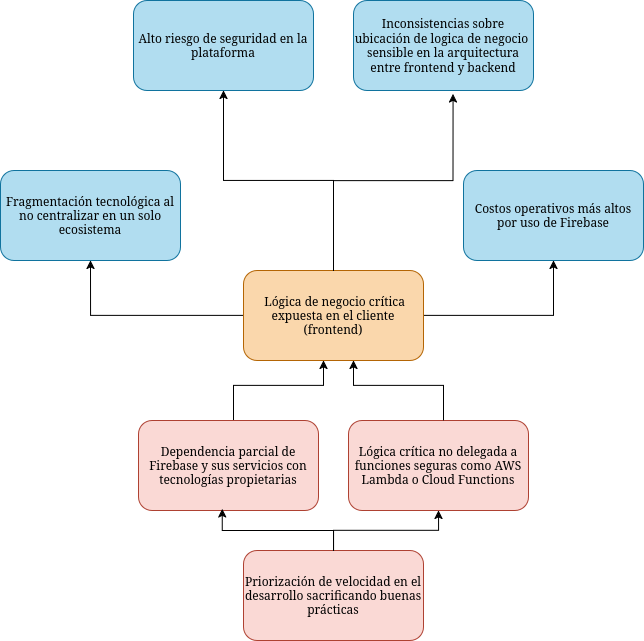
\includegraphics[width=0.85\textwidth]{img/figures/fig2-arbol-de-problemas.png}
  \caption[\captionArbolProblemas]{\captionArbolProblemas Fuente: Elaboración Propia.}
  \label{fig:arbol_problemas}
\end{figure}

\subsection{Definición del Problema}
A partir del análisis realizado, se plantea como problema central a resolver el siguiente:
\begin{quote}
  \textbf{¿Cómo migrar y adaptar la infraestructura de la plataforma Paralegales desde Firebase hacia AWS de manera que se mejore la seguridad, se elimine la exposición de lógica crítica en el cliente, se reduzcan los costos operativos y se optimice la escalabilidad y mantenibilidad del sistema?}
\end{quote}

De este problema principal se derivan las siguientes preguntas específicas:

\begin{enumerate}
  \item \textbf{¿Qué servicios de AWS pueden reemplazar adecuadamente los servicios actuales de Firebase utilizados en Paralegales?}
  \item \textbf{¿Qué estrategias de migración permiten trasladar de forma segura y eficiente tanto los datos almacenados en la base de datos como los registros de usuarios desde Firebase hacia AWS, minimizando el impacto operativo?}
  \item \textbf{¿Cómo puede estructurarse una arquitectura basada en AWS que mejore la seguridad y reduzca la fragmentación tecnológica?}
  \item \textbf{¿Qué enfoques técnicos y metodológicos deben adoptarse durante el proceso de migración para garantizar la integridad de los datos y la continuidad del servicio?}
  \item \textbf{¿Qué medidas deben tomarse para optimizar los costos en AWS sin comprometer la calidad del servicio?}
\end{enumerate}

Estas preguntas guiarán el desarrollo del proyecto y permitirán estructurar un plan de migración que no solo atienda las necesidades actuales, sino que también prepare a la plataforma para un crecimiento seguro y sostenible.

\section{Marco de Referencia}
\subsection{Marco Conceptual}

\subsubsection{Computación en la Nube}

"La computación en la nube es un modelo que permite el acceso ubicuo, conveniente y bajo demanda a un conjunto compartido de recursos de computación configurables, los cuales pueden ser rápidamente provisionados y liberados con una mínima gestión o interacción con el proveedor de servicios" \cite{Mell2011}. Este modelo ofrece beneficios significativos como elasticidad, pago por consumo y alta disponibilidad, factores esenciales en la modernización de plataformas como Paralegales.

La computación en nube se puede clasificar en modelos de servicio. Entre los cuales se destacan: \textit{Software as a Service} (SaaS), \textit{Platform as a Service} (PaaS), \textit{Infrastructure as a Service} (IaaS), \textit{Backend as a Service} (BaaS), etc \cite{Mell2011}. BaaS, ofrece a los desarrolladores funcionalidades listas para usar, como bases de datos, autenticación, almacenamiento de archivos, notificaciones \textit{push}, etc. Sin necesidad de gestionar servidores o infraestructura, por medio de un SDK. Firebase, utilizado en la etapa inicial de Paralegales es un ejemplo de BaaS. Por otro lado, Paralegales también hace uso de algunos servicios bajo el modelo \textit{Function as a Service} (FaaS), como es el caso de AWS Lambda.

\subsubsection{Vendor Lock-in}

En el contexto de la computación en nube, el término \textit{vendor lock-in} se refiere a la dificultad de cambiar de proveedor de servicios una vez que una organización ha adoptado una plataforma específica.  Esta dependencia puede deberse a diversos factores, tales como los altos costos de migración de datos, la utilización de interfaces de programación de aplicaciones (APIs) propietarias o incompatibles con estándares abiertos, y la integración profunda con servicios específicos del proveedor. Según \textcite{OparaMartins2016}, esta dependencia puede llevar a limitaciones en la portabilidad de aplicaciones, mayores costos a largo plazo y una menor capacidad de adaptación a nuevas tecnologías. En el caso de Paralegales, la alta dependencia del ecosistema Firebase representa un riesgo estratégico que se busca mitigar mediante la migración hacia AWS.

\subsubsection{Arquitectura de Software en la Nube}

El diseño de arquitecturas robustas y escalables en la nube requiere la aplicación de buenas prácticas reconocidas internacionalmente. AWS propone el Well-Architected Framework, que establece principios fundamentales para la creación de sistemas seguros, eficientes y resilientes \cite{AWS2024}. Este marco guía la toma de decisiones en áreas como seguridad, fiabilidad, eficiencia en el rendimiento, optimización de costos y excelencia operativa, todos ellos factores considerados para la nueva arquitectura de Paralegales.

\subsubsection{Seguridad en aplicaciones Web}

Garantizar la seguridad de las aplicaciones web es un desafío creciente en el entorno tecnológico actual. El OWASP Top 10 identifica las principales amenazas de seguridad, incluyendo \textit{Insecure Design}, que se refiere a deficiencias estructurales en la arquitectura de software que permiten vulnerabilidades explotables \cite{OWASP2021}. La exposición de lógica de negocio crítica en el \textit{frontend}, como ocurre actualmente en Paralegales, constituye un ejemplo claro de esta categoría de riesgo.

\subsubsection{Patrones de Diseño y Mejores Prácticas}

En el desarrollo de soluciones tecnológicas robustas y escalables, la adopción de patrones de diseño y mejores prácticas constituye una pieza clave para garantizar la calidad del software, su mantenibilidad y su evolución futura. A lo largo de los años, la comunidad de ingeniería de software ha establecido enfoques estandarizados que ayudan a resolver problemas comunes de forma reutilizable y comprensible.

Uno de los grupos más influyentes en este ámbito es el de los denominados \textit{"Gang of Four"} (GoF), quienes documentaron 23 patrones de diseño orientados a objetos (OOP) ampliamente utilizados \cite{Gamma1994}. Martin Fowler \cite{Fowler2002}, también ha contribuido significativamente con enfoques arquitectónicos y patrones de diseño. Además de los enfoques OOP, las influencias de la programación funcional (FP) han ganado terreno en arquitecturas modernas. Algunos de estos patrones están siendo usados en Paralegales, como Inyección de Dependencias, Abstract Repository Pattern, Iterator, Adapter, Closures, Funciones de Orden Superior etc.

Por otro lado, prácticas como \textit{Clean Code}, promovidas por Robert C. Martin \cite{Martin2008}, buscan mejorar la legibilidad, claridad y simplicidad del código fuente. Estas se complementan con enfoques arquitectónicos como el \textit{Domain-Driven Design} (DDD), el cual propone construir el software en torno al dominio del negocio mediante el uso de un lenguaje ubicuo y estructuras organizadas \cite{Evans2003}.

Además, la codificación de pruebas automatizadas integradas en pipelines de integración y entrega continua (CI/CD), permite asegurar calidad, reducir errores y mejorar la confiabilidad en cada fase del ciclo de vida del desarrollo de software. Junto con prácticas como el \textit{Test-Driven Development} (TDD), se promueve un desarrollo más robusto y mantenible, con menos errores y un ciclo de retroalimentación más rápido y eficiente.

\subsection{Marco Teórico}

\subsubsection{Teoría General de Sistemas}

La Teoría General de Sistemas (TGS), propuesta por Ludwig von Bertalanffy en la década de 1950, plantea que cualquier organización, fenómeno o entidad puede ser comprendida como un sistema compuesto por partes interrelacionadas que funcionan como un todo para lograr una serie de objetivos. Desde esta perspectiva, un sistema no se analiza en forma aislada, sino en términos de sus relaciones internas y su interacción con el entorno \cite{Bertalanffy1968}.

Según la TGS, todo sistema está compuesto por subsistemas interdependientes que interactúan entre sí, y a su vez forma parte de un suprasistema o entorno más amplio. Estos subsistemas intercambian información, recursos o energía a través de entradas (\textit{inputs}) y salidas (\textit{outputs}), y buscan mantener un estado de equilibrio dinámico para adaptarse a cambios en el entorno \cite{Bertalanffy1968}. Los principios de retroalimentación, homeostasis, equifinalidad y sinergia son claves para entender el comportamiento sistémico.

En este contexto, Paralegales como proyecto de Software puede concebirse como un sistema socio-técnico complejo, compuesto por diversos subsistemas funcionales: el \textit{backend}, el \textit{frontend}, la base de datos, la infraestructura en la nube, los usuarios y el equipo de desarrolladores, los stakeholders, etc.

La decisión de migrar de Firebase a AWS se fundamenta, desde la TGS, en la necesidad de reconfigurar el sistema para mejorar su capacidad de adaptación y evolución. Al adoptar modelos como BaaS, FaaS e infraestructura modular que reemplacen la dependencia de Firebase, se busca lograr una arquitectura más abierta, flexible y mantenible, que facilite la interacción eficiente entre los subsistemas y responda mejor a los cambios del entorno organizacional y tecnológico.

Asimismo, el enfoque sistémico permite identificar interdependencias críticas, como la coordinación entre equipos, la automatización del despliegue de software (CI/CD), la integración de servicios distribuidos. En la organización del código fuente, permite analizar las dependencias entre los componentes, abstracciones, acoplamiento, etc. Todo esto permite al sistema Paralegales alcanzar una mayor resiliencia y avanzar hacia un estado de equilibrio más robusto y sostenible.

\subsection{Estado del Arte}

\subsubsection{Migración de plataformas Firebase hacia arquitecturas en AWS}

Como lo indica J. Michel \cite{Michael2021}, Firebase ofrece una arquitectura de dos capas, donde las aplicaciones cliente (web o móviles) interactúan directamente con servicios \textit{backend} como Firestore, Authentication y Cloud Functions. Esta simplicidad facilita el desarrollo rápido de MVPs, pero puede presentar desafíos en escalabilidad, control y flexibilidad a medida que la aplicación crece. Obsérvese la \autoref{fig:firebase_architecture}.

\newcommand\firebaseArchitectureCaption{Diagrama de Arquitectura de Firebase. \hspace{1em}}

\begin{figure}[H]
  \centering
  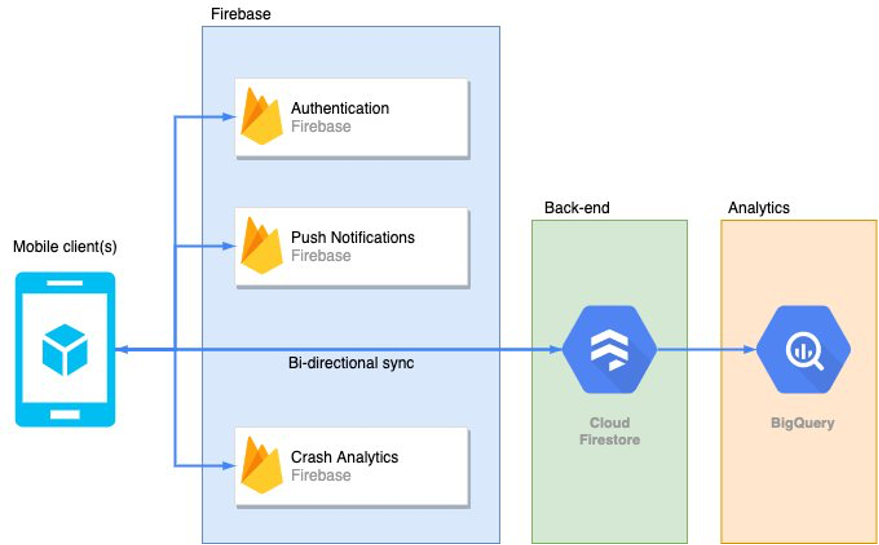
\includegraphics[width=0.7\textwidth]{img/figures/fig3-firebase-architecture.png}
  \caption[\firebaseArchitectureCaption]{\firebaseArchitectureCaption Fuente: Tomado de \cite{Michael2021}.}
  \label{fig:firebase_architecture}
\end{figure}

En contraste, como se muestra en la \autoref{fig:amplify_architecture}, AWS adopta una arquitectura de tres capas, donde se separan de forma clara la capa de presentación, la lógica de negocio y la capa de datos. Esta organización modular permite un mayor control, escalabilidad y mantenibilidad del sistema, además de reducir significativamente el riesgo de exponer lógica de negocio crítica en el cliente.

En este enfoque, el cliente utiliza el SDK de AWS Amplify para comunicarse con los servicios del \textit{backend}, los cuales están implementados mediante funciones Lambda, las cuales pueden ser accedidas mediante una API REST usando Amazon API Gateway. De esta forma, se evita el acceso directo desde el frontend a las bases de datos o a la lógica sensible del negocio, incrementando la seguridad y permitiendo una evolución más controlada de la arquitectura.

\newcommand\AWSDiagramaArquitecturaCaption{Diagrama de Arquitectura de AWS Amplify. \hspace{1em}}

\begin{figure}[H]
  \centering
  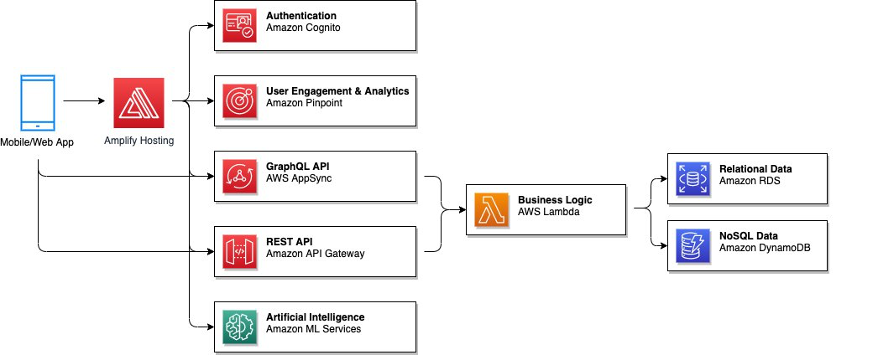
\includegraphics[width=1\textwidth]{img/figures/fig4-amplify-architecture.png}
  \caption[\AWSDiagramaArquitecturaCaption]{\AWSDiagramaArquitecturaCaption Fuente: Tomado de \cite{Michael2021}}
  \label{fig:amplify_architecture}
\end{figure}

A diferencia de Firebase, donde todos los servicios están integrados dentro de una misma plataforma, AWS ofrece un enfoque más flexible y modular. Herramientas como AWS Amplify y el Amazon Cloud Development Kit (CDK) permiten definir, configurar e implementar servicios \textit{backend} de forma personalizada \cite{Michael2021}. Amplify proporciona un conjunto de herramientas para el desarrollo, incluyendo SDKs, generación automática de código y una pipeline DevOps que facilita la integración entre los servicios de AWS y las aplicaciones web o móviles \cite{Michael2021}.

Este enfoque permite construir arquitecturas completamente adaptadas a las necesidades del proyecto, seleccionando únicamente los servicios requeridos. Además, gracias al uso de Infraestructura como Código (IaC) mediante CDK o CloudFormation, es posible versionar, reutilizar y automatizar la configuración de los recursos, mejorando la mantenibilidad y escalabilidad del sistema.

Por otro lado, la migración de Firebase a AWS implica identificar servicios equivalentes que ofrezcan funcionalidades similares, pero con mayor flexibilidad y escalabilidad. La \autoref{tab:aws_firebase_comparison_services} presenta la correspondencia general entre servicios de Firebase y sus equivalentes en AWS.

\newcommand\correspondenciaFirebaseAWSCaption{Correspondencia general entre los servicios de Firebase y sus equivalentes en AWS. \hspace{1em}}
\begin{table}[H]
  \centering
  \begin{tabular}{|l|l|}
    \hline
    \grayTableHeaderCell{6cm}{Funcionalidad Firebase} & \grayTableHeaderCell{8cm}{Servicio AWS Equivalente} \\

    \hline
    Firebase Authentication & Amazon Cognito \\
    \hline
    Cloud Firestore & Amazon DynamoDB \\
    \hline
    Firebase Cloud Functions & AWS Lambda \\
    \hline
    Firebase Cloud Messaging & Amazon SNS \\
    \hline
    Cloud Storage & Amazon S3 + Amazon CloudFront \\
    \hline
    Firebase Hosting & AWS Amplify \\
    \hline
  \end{tabular}
  \caption[\correspondenciaFirebaseAWSCaption]{\correspondenciaFirebaseAWSCaption Fuente: Elaboración propia.}
  \label{tab:aws_firebase_comparison_services}
\end{table}

Esta correspondencia permite a las aplicaciones migradas beneficiarse de la robustez y escalabilidad de los servicios de AWS, adaptándose mejor a las necesidades empresariales en crecimiento.

Actualmente, la plataforma de Paralegales utiliza únicamente algunos servicios clave de Firebase: Firebase Authentication para la gestión de usuarios, Cloud Firestore como base de datos NoSQL y lógica de negocio crítica implementada directamente en el cliente. Esta última representa un riesgo de seguridad, ya que expone operaciones sensibles en el frontend. Como parte del proceso de migración a AWS, estos componentes serán reemplazados por servicios equivalentes más robustos y seguros: Amazon Cognito asumirá la autenticación de usuarios, Amazon DynamoDB gestionará los datos, y la lógica de negocio crítica será trasladada a funciones AWS Lambda, ejecutadas desde el \textit{backend}.

La migración de una plataforma desde Firebase a AWS requiere una planificación cuidadosa para minimizar interrupciones, preservar la integridad de los datos y garantizar una experiencia fluida para los usuarios. En el caso de Paralegales, esta transición está prevista una vez que la aplicación esté en producción y cuente con usuarios reales, lo que hace aún más crucial la implementación de estrategias que permitan una migración progresiva y controlada. A continuación, se describen las principales estrategias consideradas para llevar a cabo este proceso.

\subsubsection{Migración de usuarios de Firebase a Amazon Cognito}

Como lo indica A. Hall en el blog de AWS \cite{Hall2017}, Existen dos métodos principales para migrar usuarios:

\begin{enumerate}[label=\alph*)]

\item \textbf{\textit{Importación por lotes}}: Consiste en exportar los datos de usuario desde Firebase y cargarlos en Amazon Cognito mediante un archivo CSV. Es importante destacar que las contraseñas no se migran, por lo que los usuarios deberán restablecerse al iniciar sesión por primera vez en el nuevo sistema.

\item \textbf{\textit{Migración individual al iniciar sesión}}: Esta estrategia permite migrar usuarios a medida que inician sesión. Si un usuario no existe en Cognito, se autentica mediante Firebase y luego se crea su cuenta en Cognito, permitiendo una transición sin interrupciones para el usuario.
\end{enumerate}

\subsubsection{Migración de datos de Firestore a DynamoDB}

La migración de datos puede realizarse mediante los siguientes enfoques complementarios:

\begin{enumerate}[label=\alph*)]
\item \textbf{\textit{Carga Masiva}}: La migración de datos desde Cloud Firestore hacia Amazon DynamoDB requiere más que una simple operación de exportación e importación, ya que los modelos de datos de ambas bases de datos no son completamente compatibles. Por ello, se recomienda implementar una pipeline de tipo ETL (\textit{Extract, Transform, Load}) que permita transformar y adaptar los datos durante el proceso de migración \cite{Michael2021}.

\hfill

Esta pipeline puede construirse utilizando servicios totalmente gestionados de AWS, como AWS Step Functions para la orquestación del flujo, AWS Lambda para ejecutar cada una de las etapas del proceso de extracción, transformación y carga, y Amazon SQS para manejar la comunicación entre pasos mediante colas de mensajes. Este enfoque garantiza durabilidad y capacidad de re-ejecución de los trabajos en caso de fallos, a la vez que minimiza la carga operativa y reduce los costos al utilizar servicios \textit{serverless} \cite{Michael2021}.

\item \textbf{\textit{Sincronización en Paralelo}}: Durante un período de transición, operar ambas bases de datos en paralelo, sincronizando los cambios en tiempo real para garantizar la consistencia de los datos hasta completar la migración.
\end{enumerate}

\subsubsection{Referencia práctica de migración: implementación basada en AWS CDK}

Además de la documentación oficial, B. Shank \cite{Shank2021}, Sr. Startup SA en AWS, implementó un repositorio de código abierto en en AWS CDK que puede servir como guía práctica para realizar la migración. Dicho repositorio, incluye dos fases de despliegue y múltiples \textit{stacks} que replican los servicios clave de Firebase: Firestore, Authentication y Cloud Storage, utilizando sus equivalentes en AWS (DynamoDB, Cognito y S3, respectivamente).

\newcommand\DiagramaMigracionAWSCaption{Diagrama de Infraestructura de la migración propuesta por B. Shank. \hspace{1em}}
\begin{figure}[H]
\centering
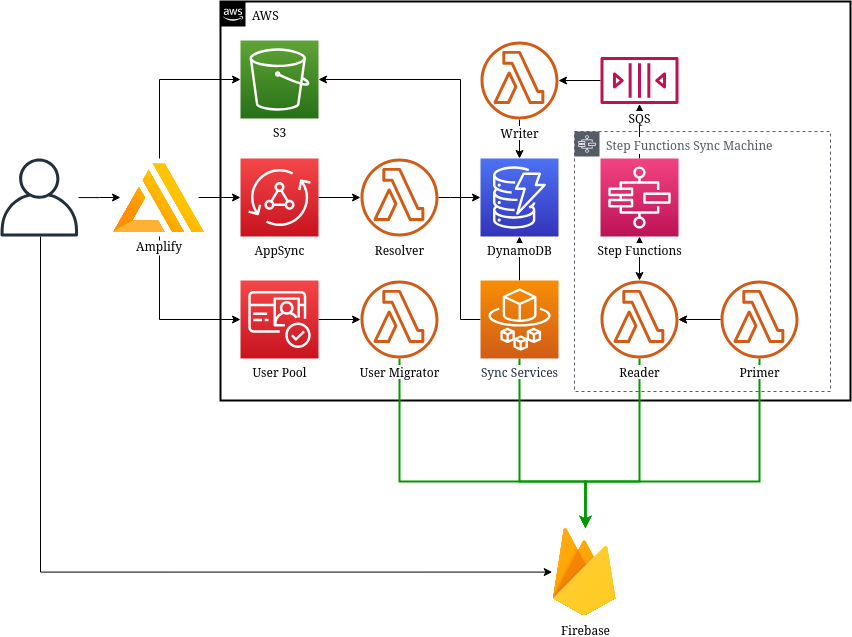
\includegraphics[width=0.9\textwidth]{img/figures/fig5-etl-pipeline-aws.png}
\caption[\DiagramaMigracionAWSCaption]{\DiagramaMigracionAWSCaption Fuente: Tomado de \cite{Shank2021}.}
\label{fig:aws_migration_pipeline}
\end{figure}

En la primera fase ilustrada en la \autoref{fig:aws_migration_pipeline}, se aprovisionan los recursos base y se ejecuta automáticamente una máquina de estados de AWS Step Functions que extrae y transforma los datos desde Firestore para cargarlos en DynamoDB, utilizando un esquema de tabla única. En paralelo, los usuarios de Firebase Authentication se migran a Amazon Cognito a través de un trigger Lambda específico durante el despliegue.

La segunda, también detallada en la \autoref{fig:aws_migration_pipeline}, fase despliega una API GraphQL con AppSync, cuya definición se genera automáticamente a partir de los datos sincronizados. También incluye un servicio en AWS Fargate que escucha eventos en tiempo real desde Firestore y sincroniza los cambios con DynamoDB. Esta arquitectura híbrida permite mantener ambas plataformas operando en paralelo durante el proceso de transición, lo que resulta especialmente útil para reducir el riesgo al migrar una aplicación en producción.

\subsubsection{Bibliografía Complementaria}
Como complemento a los enfoques técnicos revisados, el trabajo de \textcite{Kansara2024} aporta una visión más amplia sobre los desafíos y metodologías emergentes en procesos de migración de bases de datos hacia la nube. Su estudio enfatiza la automatización, la integridad de los datos y la optimización del rendimiento como pilares fundamentales para garantizar migraciones eficientes y seguras. En particular, el autor presenta un diagrama de alto nivel que descompone el proceso en fases estructuradas: extracción y validación de datos, refactorización de lógica de negocio, transferencia segura y orquestación de servicios en la nube. Esta representación, ilustrada en la \autoref{fig:etl_process_diagram}, proporciona un marco útil para entender la transición desde arquitecturas legadas hacia entornos escalables y distribuidos basados en servicios nativos de la nube.

\newcommand\migrationProcessDiagramCaption{Diagrama del proceso de migración a base de datos en la nube. \hspace{1em}}
\begin{figure}[H]
\centering
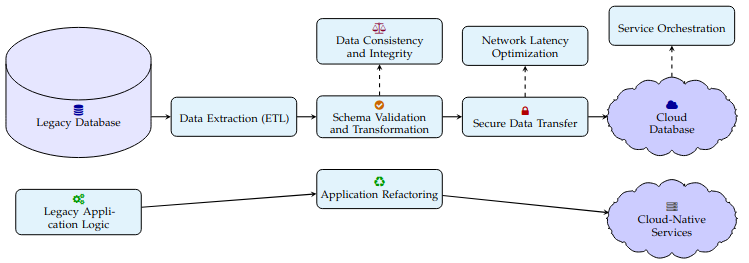
\includegraphics[width=1\textwidth]{img/figures/fig6-etl-process.png}
\caption[\migrationProcessDiagramCaption]{\migrationProcessDiagramCaption Fuente: Tomado de \cite{Kansara2024}.}
\label{fig:etl_process_diagram}
\end{figure}

Por otro lado, en la literatura complementaria se encuentra el trabajo de \textcite{Kyadasu2025}, quienes, a través de un estudio de caso sobre migración entre proveedores de nube, explican cómo las prácticas DevOps, con su enfoque en la automatización y la integración y entrega continuas (CI/CD), ofrecen beneficios significativos y presentan lo que consideran como mejores prácticas para llevar a cabo este tipo de procesos.


\section{Alcance del Proyecto}

\subsection{Declaración de Alcance del Proyecto}

Este proyecto contempla la migración y adaptación de los componentes de software en Paralegales que actualmente dependen de Firebase, ya sea para autenticación o como base de datos (Firestore), hacia servicios equivalentes en AWS. El enfoque principal estará en funcionalidades clave como autenticación, almacenamiento y gestión de datos, con el objetivo de fortalecer la arquitectura técnica de la plataforma.

Como se puede apreciar en la \autoref{fig:arbol_de_objetivos}, esta migración busca reducir la exposición de lógica crítica en el \textit{frontend} mediante su delegación a entornos seguros del \textit{backend}, como AWS Lambda. Esto permitirá mejorar aspectos fundamentales como la seguridad, la definición clara de responsabilidades arquitectónicas, y la reducción de costos operativos derivados del uso de tecnologías propietarias.

Además, como se refleja en los niveles inferiores del árbol, la propuesta fomenta la adopción de servicios equivalentes en AWS y el seguimiento de buenas prácticas de desarrollo, priorizando la calidad técnica y la sostenibilidad del sistema por encima de la velocidad en la entrega.

Asimismo, esta reestructuración permitirá avanzar hacia una homogeneización tecnológica dentro de un ecosistema centralizado, lo que facilitará la escalabilidad, el mantenimiento y la integración de los distintos componentes de la plataforma.

Quedan excluidas del alcance en esta fase la migración de herramientas como Firebase Analytics o el sistema de mensajería \textit{push}, al no formar parte del núcleo funcional contemplado en esta etapa del proyecto.

\begin{figure}[H]
  \centering
  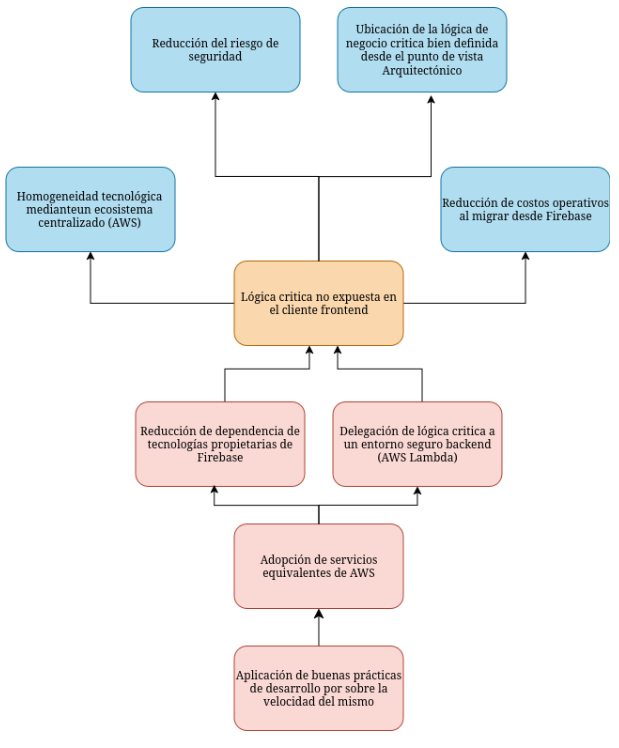
\includegraphics[width=0.85\textwidth]{img/figures/fig7-arbol-de-objetivos.png}
  \caption{Árbol de objetivos. Fuente: Elaboración Propia.}
  \label{fig:arbol_de_objetivos}
\end{figure}

\input{sections/5-alcance-del-proyecto-sub-sections/5.2-objetivos.tex}

\section{Metodologías}

\subsection{Metodología de Investigación}

Este proyecto se enmarca dentro de una metodología de investigación aplicada de base tecnológica, dado que se centra en la migración e implementación de una infraestructura tecnológica avanzada para una organización real, aplicando conocimientos previos en nuevas condiciones y validando soluciones en entornos operativos. En este tipo de investigación, el conocimiento se genera a partir de la aplicación práctica de soluciones técnicas, con énfasis en el desarrollo, validación y mejora de tecnologías existentes, más que en la formulación de teorías abstractas.

Como se puede apreciar en la \autoref{fig:tlr_levels}, se hace uso del enfoque de Niveles de Maduración Tecnológica (TLR) --\textit{Technology Readiness Level}, por sus siglas en inglés-- adoptado por Colciencias para definir el alcance y la madurez tecnológica de actividades que tienen que ver con Investigación, Desarrollo Tecnológico e Innovación ($I+D+i$) en el Sistema Nacional de Ciencia, Tecnología e Innovación (SNCTeI) en Colombia \cite{Colciencias2016}.

\begin{figure}[H]
  \centering
  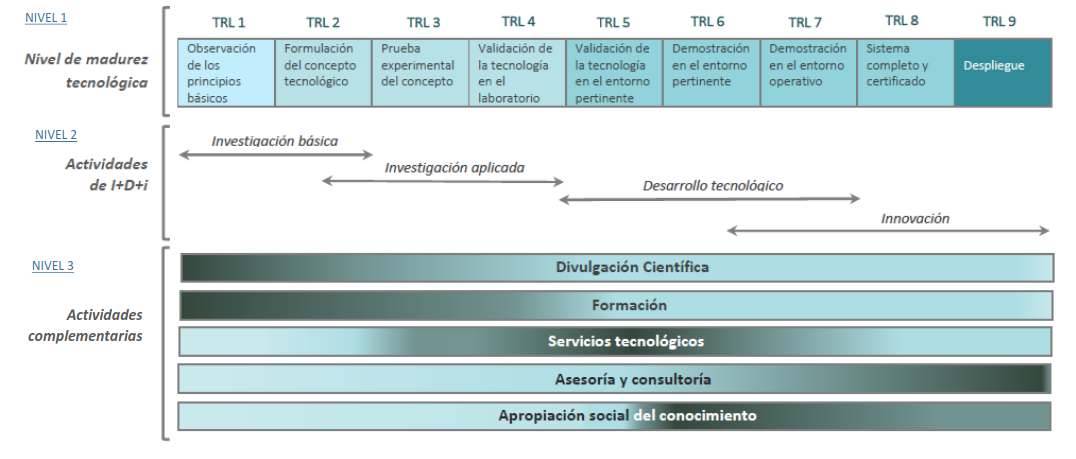
\includegraphics[width=1\textwidth]{img/figures/fig8-TLR-explanation.png}
  \caption{actividades de $I+D+i$ y otras actividades. Fuente: Tomado de \cite{Colciencias2016}}
  \label{fig:tlr_levels}
\end{figure}

Los proyectos de software como Paralegales se ubican en los niveles más altos de madurez tecnológica: TRL 7 a TRL 9, correspondientes a las fases de investigación aplicada, desarrollo tecnológico e innovación. En estos niveles se realiza la demostración de la tecnología en entornos operativos, la validación completa del sistema y su despliegue final en condiciones reales de funcionamiento.

Esta clasificación refleja con claridad el tipo de trabajo que se está llevando a cabo: una solución concreta que busca resolver problemas técnicos y operativos reales en una organización, a través de la aplicación de buenas prácticas de ingeniería de software, la integración de servicios tecnológicos avanzados y la validación continua en producción.

Por otro lado, la investigación se puede clasificar como \textit{``in vivo''} pues se desarrolla en una organización real \cite{ChavarriagaLIDIS}. Además, se opta por la estrategia de investigación definida por Chavarriaga y Arboleda, basada en los modelos de Martin y McClure, y del SEI (\textit{Software Engineering Institute}), la cual consiste en tres etapas: (1) investigación y desarrollo inicial, (2) Investigación aplicada, y (3) Transferencia \cite{ChavarriagaLIDIS,ChavarriagaModelo}.

\begin{figure}[H]
  \centering
  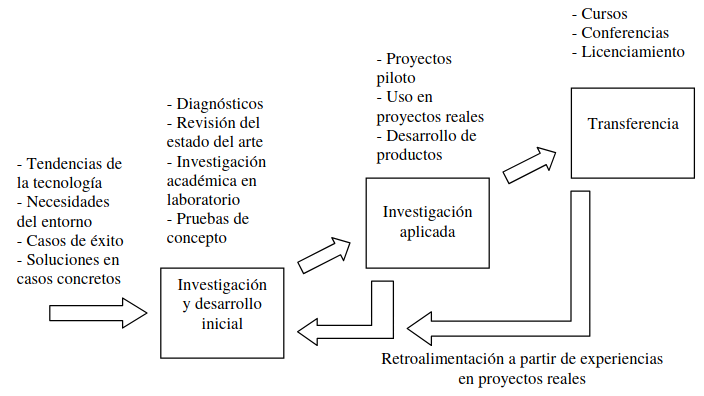
\includegraphics[width=0.8\textwidth]{img/figures/fig9-chavarriaga-arboleda.png}
  \caption{Esquema de la estrategia de investigación propuesto por Chavarriaga y Arboleda. Fuente: Tomado de \cite{ChavarriagaLIDIS}}
  \label{fig:arboleda-chavarriaga-metodologia}
\end{figure}

Como se puede apreciar en la \autoref{fig:arboleda-chavarriaga-metodologia}, el modelo parte de una fase inicial en la que se realiza un diagnóstico, revisión del estado del arte y pruebas de concepto, seguida de una etapa de investigación aplicada donde se desarrollan soluciones en escenarios reales, y finalmente se alcanza la fase de transferencia, en la cual los conocimientos y productos generados son compartidos a través de formación, licenciamiento o difusión. Esta secuencia metodológica resulta pertinente para el presente proyecto, dado que:

\begin{enumerate}
  \item Se parte de necesidades concretas del entorno (el caso de Paralegales y su infraestructura actual).
  \item Se aplican tecnologías maduras mediante pruebas controladas y despliegues en producción.
  \item Se espera generar una solución replicable, que pueda ser transferida como buena práctica en entornos similares.
\end{enumerate}

En este sentido, el proyecto no se limita al desarrollo técnico, sino que busca una contribución tecnológica efectiva, orientada a la solución de un problema real, con posibilidad de transferencia y aprovechamiento del conocimiento en otros contextos organizacionales o académicos.

\subsection{Metodología de Desarrollo de Software}

Dado que el proyecto consiste en la migración y adaptación tecnológica de una plataforma ya funcional, se requiere una metodología ágil que permita implementar mejoras continuas, validar cambios técnicos y mantener una alta calidad en el software sin perder flexibilidad. Por ello, este trabajo de grado adopta los principios y valores definidos en el Manifiesto Ágil \cite{AgileManifesto2001}. Para tomar una decisión fundamentada, se realizó una comparación multicriterio entre tres paradigmas populares de desarrollo ágil: SCRUM, que se clasifica como un marco de trabajo \cite{ScrumGuide2020}; y \textit{Extreme Programming} (XP) junto con \textit{Feature-Driven Development} (FDD), ambas reconocidas como metodologías de desarrollo.

% -- Table Setup --
\newcommand{\comparativaMetodologiasHeader}{
  \grayTableHeaderCell{3cm}{Criterio} &
  \grayTableHeaderCell{3cm}{SCRUM} &
  \grayTableHeaderCell{3cm}{XP} &
  \grayTableHeaderCell{3cm}{FDD} \\
}

\renewcommand{\arraystretch}{1.4}
\begingroup
\scriptsize
\begin{longtable}{|
    >{\raggedright\arraybackslash}p{3cm}|
    >{\raggedright\arraybackslash}p{3cm}|
    >{\raggedright\arraybackslash}p{3cm}|
    >{\raggedright\arraybackslash}p{3cm}|
  }
  \hline

  % Table Header
  \comparativaMetodologiasHeader
  \hline
  \endfirsthead

  % Encabezado para las siguientes páginas:
  \hline
  \comparativaMetodologiasHeader
  \hline
  \endhead

  \continuacionTablaFooter{4}
  \endfoot
  \endlastfoot

  % Table Body
  \tableCell{ Orientación } &
  \tableCell{ Gestión de proyectos iterativa basada en roles y eventos } &
  \tableCell{ Desarrollo técnico intensivo con foco en calidad del código } &
  \tableCell{Desarrollo centrado en funcionalidades del sistema } \\
  \hline

  \tableCell{ Planificación} &
  \tableCell{ Sprint Planning, backlog de producto y de sprint } &
  \tableCell{ Historias de usuario, planificación continua } &
  \tableCell{ Modelo inicial y listado detallado de features } \\
  \hline

  \tableCell{ Iteraciones } &
  \tableCell{ Sprints de 1 a 4 semanas } &
  \tableCell{ Iteraciones muy cortas (1 semana o menos) } &
  \tableCell{ Iteraciones basadas en funcionalidades } \\
  \hline

  \tableCell{ Control de calidad } &
  \tableCell{ Revisión de sprint, retrospectivas, testing por parte del equipo } &
  \tableCell{ Desarrollo guiado por pruebas (TDD), integración continua, pair programming } &
  \tableCell{ Enfoque más estructurado y menos centrado en pruebas } \\
  \hline

  \tableCell{ Tamaño del equipo recomendado } &
  \tableCell{ menos de 10 personas \cite{ScrumGuide2020}. } &
  \tableCell{ Equipos pequeños y altamente colaborativos } &
  \tableCell{ Equipos más grandes con roles definidos (desarrolladores, arquitectos, modeladores) } \\
  \hline

  \tableCell{ Adecuación al proyecto de migración } &
  \tableCell{ Buena para seguimiento y coordinación, pero requiere adaptación técnica adicional } &
  \tableCell{ Excelente por su enfoque técnico (ideal para migración de lógica crítica y refactorización) }&
  \tableCell{ Menos adecuado en etapas tempranas o de reestructuración } \\
  \hline

  \tableCell{ Documentación } &
  \tableCell{ Ligeramente documentado, foco en entregables funcionales } &
  \tableCell{ Baja formalidad documental, más foco en código limpio } &
  \tableCell{ Documentación moderada y estructurada } \\
  \hline

  \tableCell{ Entrega de valor } &
  \tableCell{ Al final de cada sprint } &
  \tableCell{ Entregas muy frecuentes (incluso diarias) } &
  \tableCell{ Entrega continua por funcionalidad } \\
  \hline

  \caption{Comparativa entre las metodologías de desarrollo de software de interés. Fuente: Elaboración propia.}
  \label{tab:comparativa_metodologias}
\end{longtable}
\endgroup

Como se puede observar en la \autoref{tab:comparativa_metodologias}, tanto SCRUM como XP se ajustan bien al contexto del proyecto actual. Sin embargo, SCRUM destaca por su estructura ligera pero efectiva para la planificación y seguimiento, especialmente útil dado que el equipo de Paralegales ya trabaja con iteraciones, reuniones de revisión y planificación de manera semanal. Además, su claridad de roles y enfoque incremental permiten mantener un flujo de trabajo ordenado y adaptativo \cite{ScrumGuide2020}.

Por estas razones, SCRUM ha sido seleccionada como la metodología base para el desarrollo del software en este proyecto. No obstante, se complementará con prácticas de XP, como TDD y \textit{pair programming}, cuando sea pertinente, para mejorar la calidad del código y la colaboración técnica.

Adicionalmente, el proyecto busca adoptar progresivamente una cultura DevOps, integrando prácticas como la contribución continua a los repositorios de código, automatización de pruebas y despliegues, y un enfoque centrado en la seguridad, trazabilidad y control del ciclo de vida del software. Estas prácticas, alineadas con principios de integración y entrega continua (CI/CD) \cite{Bass2015}, ya han comenzado a ser aplicadas dentro de Paralegales y constituyen un eje fundamental para garantizar despliegues seguros y eficientes.

Finalmente, es importante enfatizar que las metodologías ágiles y marcos de trabajo no deben concebirse como estructuras rígidas o absolutas, sino como guías adaptables que deben ajustarse de forma pragmática a las características, recursos y necesidades particulares de cada proyecto \cite{BoehmTurner2004}.

\subsection{Metodología de Gestión de Actividades}

La gestión de actividades se articula directamente con SCRUM, el cual fue seleccionado como el marco de trabajo que guiará la metodología de desarrollo de software. Bajo este enfoque el proyecto se organiza en iteraciones semanales fijas.

Para la planificación y control del trabajo se hace uso de un software interno de gestión de actividades, en el cual se encuentra el \textit{backlog} del producto, que representa el conjunto de tareas pendientes. A partir de este \textit{backlog}, se seleccionan las tareas y funcionalidades a priorizar en cada \textit{sprint} mediante una reunión sincrónica con el equipo (Desarrolladores, \textit{Product Owner} y  \textit{Tech Lead}). Adicionalmente, se utiliza un tablero Kanban como apoyo visual para facilitar el seguimiento del estado de cada tarea en tiempo real.

Por otro lado, la comunicación sincrónica se gestiona mediante Google Meet para realizar el sprint planning y Discord usado por el equipo de desarrollo para hacer Pair Programming y Revisión de código. La comunicación asincrónica se gestiona principalmente mediante Telegram y WhatsApp, herramientas que permiten mantener una interacción constante entre los miembros del equipo.


\section{Programa de Hitos}

Con se mostró en el marco lógico, las siguientes son las actividades relacionadas a cada objetivo especifico.

\textbf{Objetivo 1:} \objetivoEspecificoA
\objetivoEspecificoAActividades

\textbf{Objetivo 2:} \objetivoEspecificoB
\objetivoEspecificoBActividades

\textbf{Objetivo 3:} \objetivoEspecificoC
\objetivoEspecificoCActividades

\textbf{Objetivo 4:} \objetivoEspecificoD
\objetivoEspecificoDActividades

\textbf{Actividad 1:} \objetivoEspecificoDocument
\objetivoEspecificoDocumentActividades

\begin{table}[H]
  \small
  \centering
  \begin{tabular}{|p{5cm}|c|c|c|c|c|c|c|c|}
    \hline
    \grayTableHeaderCell{5cm}{Actividad} &
    \grayTableHeaderCell{1cm}{Mes 1} &
    \grayTableHeaderCell{1cm}{Mes 2} &
    \grayTableHeaderCell{1cm}{Mes 3} &
    \grayTableHeaderCell{1cm}{Mes 4} &
    \grayTableHeaderCell{1cm}{Mes 5} &
    \grayTableHeaderCell{1cm}{Mes 6} &
    \grayTableHeaderCell{1cm}{Mes 7} &
    \grayTableHeaderCell{1cm}{Mes 8} \\

    \hline
    1.1 \objectivoEspecificoAActividadadA & X & & & & & & & \\
    \hline
    1.2 \objectivoEspecificoAActividadadB & X & & & & & & & \\
    \hline
    1.3 \objectivoEspecificoAActividadadC & & X & & & & & & \\
    \hline
    1.4 \objectivoEspecificoAActividadadD & & X & & & & & & \\
    \hline

    2.1 \objectivoEspecificoBActividadadA & & & X & & & & & \\
    \hline
    2.2 \objectivoEspecificoBActividadadB & & & X & X & & & & \\
    \hline
    2.3 \objectivoEspecificoBActividadadC & & & X & X & & & & \\
    \hline
    2.4 \objectivoEspecificoBActividadadD & & & X & X & & & & \\
    \hline

    3.1 \objectivoEspecificoCActividadadA & & & & & X & & & \\
    \hline
    3.2 \objectivoEspecificoCActividadadB & & & & & X & & & \\
    \hline
    3.3 \objectivoEspecificoCActividadadC & & & & & & X & X & \\
    \hline
    3.4 \objectivoEspecificoCActividadadD & & & & & & X & X & \\
    \hline

    4.1 \objectivoEspecificoDActividadadA & & X & X & X & X & X & X & \\
    \hline
    4.2 \objectivoEspecificoDActividadadB & & X & X & X & X & X & X & \\
    \hline
    4.3 \objectivoEspecificoDActividadadC & & X & X & & & & & \\
    \hline
    4.4 \objectivoEspecificoDActividadadD & & X & X & X & X & X & X & \\
    \hline

    A.1 \objetivoEspecificoDocumentActividadA & X & X & X & X & X & X & & \\
    \hline
    A.2 \objetivoEspecificoDocumentActividadB & & & X & X & X & X & X & \\
    \hline
    A.3 \objetivoEspecificoDocumentActividadC & & & & & & & & X \\
    \hline

  \end{tabular}
  \caption{Cronograma de actividades. Fuente: Elaboración propia.}
  \label{tab:cronograma-actividades}
\end{table}

\section{Presupuesto}

El Trabajo de Grado, en el marco del programa de Ingeniería de Sistemas, comprende  9 créditos académicos según la Resolución 048 de abril de 2010 \cite{Univalle2010}. Con base en el Artículo 11 del Decreto 1295 de 2010 del Ministerio de Educación (MEN) \cite{MEN2010}, cada crédito equivale a 48 horas de trabajo académico. Esto totaliza 432 horas de dedicación (9 créditos $\times$ 48 horas/crédito) por parte del estudiante, incluyendo tanto el acompañamiento docente como el trabajo independiente para el desarrollo de la propuesta.

\begin{table}[H]
  \centering
  \begin{tabular}{|l|c|}
    \hline
    \grayTableHeaderCell{6cm}{Indicador} & \grayTableHeaderCell{8cm}{Valor} \\
    \hline
    Número de créditos & 9 \\
    \hline
    Horas por crédito & 48 \\
    \hline
    Total horas trabajo de grado & 432 \\
    \hline
  \end{tabular}
  \caption{Créditos y horas destinados al trabajo de grado. Fuente: elaboración propia. Fuente: Elaboración propia.}
  \label{tab:creditos_horas_trabajo_grado}
\end{table}

Además, en la Resolución 022 de 2001 de la Universidad del Valle \cite{CSUnivalle2001}, se establece que la dedicación para asesorías de trabajos de investigación de pregrado es de 22 horas semestrales por parte del director del trabajo de grado el cual dedicará 44 horas a la asesoría del estudiante. Para el cálculo de los rubros, se considerará el valor de la hora de un salario mínimo para el estudiante y el valor de la hora basada en la categoría docente para el profesor. La \autoref{tab:costos_personal_proyecto} detalla los costos asociados al personal, el valor del proyecto por costos de personal asciende a \$5'200.612 COP.

\begin{table}[H]
  \centering
  \begin{tabular}{|p{4cm}|c|c|c|}
    \hline
    \grayTableHeaderCell{4cm}{Rubro} &
    \grayTableHeaderCell{3cm}{Cantidad de horas} &
    \grayTableHeaderCell{3cm}{Valor unitario por hora} &
    \grayTableHeaderCell{3cm}{Total} \\
    \hline
    Horas profesor Asociado & 44 & \$57.431 COP & \$ 2'526.964 COP \\
    \hline
    Horas de dedicación del estudiante & 432 & \$6.189 COP & \$2'673.648 COP \\
    \hline
    Total & - & - & \$5'200.612 COP \\
    \hline
  \end{tabular}
  \caption{Costos asociados al personal del proyecto. Fuente: Elaboración propia.}
  \label{tab:costos_personal_proyecto}
\end{table}

\begin{table}[H]
  \centering
  \begin{tabular}{|p{3cm}|c|c|p{3.5cm}|}
    \hline
    \grayTableHeaderCell{3cm}{Concepto} &
    \grayTableHeaderCell{3cm}{Cantidad} &
    \grayTableHeaderCell{3cm}{Costo unitario} &
    \grayTableHeaderCell{3.5cm}{\rule{0pt}{1em}Depreciación mensual estimada \vspace{1em}} \\
    \hline

    Computador estudiante & 1 & \$3'100.000 COP & \$51.666,67 COP \\
    \hline
    Total & - & - & \$41.333,36 COP \\
    \hline

  \end{tabular}
  \caption{Costos en la depreciación de los equipos Fuente: Elaboración propia.}
  \label{tab:costos_equipo_proyecto}
\end{table}

Con base en el método de depreciación de línea recta y los 8 meses del proyecto por concepto de equipamiento el rubro alcanza los \$41.3333,36 COP.

\begin{table}[H]
  \centering
  \begin{tabular}{|p{4cm}|c|c|}
    \hline
    \grayTableHeaderCell{5cm}{Concepto} &
    \grayTableHeaderCell{5cm}{Costo unitario (8 meses)} \\
    \hline

    Servicio de Internet & \$504.000 COP \\
    \hline
    Gastos en nube (AWS + Firebase) & \$100.000 COP \\
    \hline
    Total & \$604.000 COP \\
    \hline
  \end{tabular}
  \caption{Gastos adicionales del proyecto. Fuente: Elaboración propia.}
  \label{tab:gastos_adicionales_proyecto}
\end{table}

\begin{table}[H]
  \centering
  \begin{tabular}{|p{4cm}|c|}
    \hline
    \grayTableHeaderCell{4cm}{Rubro} & \grayTableHeaderCell{3cm}{Valor} \\
    \hline
    Personal & \$5'200.612 COP \\
    \hline
    Equipamiento & \$41.3333,36 COP \\
    \hline
    Gastos Adicionales & \$604.000 COP \\
    \hline
    Total & \$5'614.549,36 COP \\
    \hline
  \end{tabular}
  \caption{Presupuesto total del proyecto de grado. Fuente: Elaboración propia.}
  \label{tab:presupuesto_total_proyecto_grado}
\end{table}

El costo total de la propuesta durante 8 meses asciende a \$5'614549.36 COP con base en la \autoref{tab:presupuesto_total_proyecto_grado}.

\section{Impacto Ambiental}

Dada la importancia de evaluar el impacto ambiental de las actividades del proyecto. Como se puede observar en la \autoref{tab:consumo_energetico_dispositivos} se procede a realizar un análisis de la huella de carbono generada por el consumo energético de los dispositivos utilizados en la operación.

% Avoid magic strings
\newcommand{\deviceAName}{ Computador principal }
\newcommand{\deviceBName}{ Monitor Sansui ES-22X3 }
\newcommand{\deviceCName}{ Conexión a internet }

\newcommand\consumoEnergeticoCaption{Consumo energético de los dispositivos. \hspace{1em}}

\begin{table}[H]
  \centering
  \begin{tabular}{|c|c|c|c|}
    \hline
    \grayTableHeaderCell{3cm}{Dispositivo} &
    \grayTableHeaderCell{3cm}{Consumo Real Promedio (Watts / hora)} &
    \grayTableHeaderCell{3cm}{Consumo en Suspensión Promedio (Watts / hora)} &
    \grayTableHeaderCell{3cm}{Consumo Apagado Promedio (Watts / hora)} \\
    \hline

    \deviceAName\footnote{El consumo del computador principal fue medido usando la herramienta \texttt{powerstat} en Linux (polyfiling).}  & 11,63 & 2,5 & 5 \\

    \deviceBName & 13,35 \cite{Device_report_sansui} & 0,5 & 1 \\
    \deviceCName & 25 & 0 & 0 \\
    \hline

    Total & 49,98 & 3,0 & 6,0 \\
    \hline
  \end{tabular}
  \caption[\consumoEnergeticoCaption]{\consumoEnergeticoCaption Fuente: Elaboración propia.}
  \label{tab:consumo_energetico_dispositivos}
\end{table}

Por otra parte, la \autoref{tab:consumo_energetico_previsto} presenta el consumo de cada dispositivo con base en las horas efectivas de trabajo previstas para las fases iniciales de la operación.

\newcommand\consumoEnergeticoPrevistoCaption{Consumo energético previsto de los dispositivos. \hspace{1em}}

\begin{table}[H]
  \centering
  \begin{tabular}{|p{3cm}|c|c|c|c|c|c|c|c|}
    \hline
    \grayTableHeaderCell{2cm}{Dispositivo} &
    \grayTableHeaderCell{2cm}{Uso normal horas / día} &
    \grayTableHeaderCell{1cm}{ (1) Kw / hora } &
    \grayTableHeaderCell{1cm}{ (2) Horas / día }  &
    \grayTableHeaderCell{1cm}{ (3) Kw / hora }  &
    \grayTableHeaderCell{1cm}{ (4) Horas / día } &
    \grayTableHeaderCell{1cm}{ (5) Kw / hora } &
    \grayTableHeaderCell{1cm}{ (6) Kw / hora } &
    \grayTableHeaderCell{1cm}{ (7) Kw / hora } \\
    \hline

    \deviceAName & 6 & 0.100 & 1 & 0.005 & 17 & 0.001 & 0.600 & 0.606 \\
    \deviceBName & 6 & 0.025 & 1 & 0.002 & 17 & 0.001 & 0.150 & 0.153 \\
    \deviceCName & 24 & 0.010 & 0 & 0.000 & 0 & 0.001 & 0.240 & 0.240 \\

    \hline
    \textbf{Total día} & - & - & - & - & - & - & \textbf{0.990} & \textbf{0.999} \\
    \hline
  \end{tabular}
  \caption[\consumoEnergeticoPrevistoCaption]{\consumoEnergeticoPrevistoCaption Fuente: Elaboración propia.}
  \label{tab:consumo_energetico_previsto}
\end{table}

\begin{itemize}
  \item (1) Consumo en condiciones de funcionamiento normal
  \item (2) Consumo en estado de suspensión o hibernado
  \item (3) Consumo en estado de apagado
  \item (4) Consumo real total al día
  \item (5) Consumo fantasma al día
\end{itemize}

Suponiendo que por semana se trabajan 5 días, se presentan los consumos semanales, fantasma, mensual y anual en la \autoref{tab:consumo_energetico_totalizado}.

\newcommand\consumoEnergeticoTotalCaption{Consumo energético totalizado. \hspace{1em}}

\begin{table}[H]
  \centering
  \begin{tabular}{|c|c|c|c|c|}
    \hline
    \grayTableHeaderCell{3cm}{Consumo Semanal (Kw/hora)} &
    \grayTableHeaderCell{3cm}{Consumo Fantasma (Kw/hora)} &
    \grayTableHeaderCell{3cm}{Consumo Mensual (Kw/hora)} &
    \grayTableHeaderCell{3cm}{Consumo Anual (Kw/hora)} \\
    \hline
    6,993 & 0,27 & 29,97 & 364,64 \\
    \hline
  \end{tabular}
  \caption[\consumoEnergeticoTotalCaption]{\consumoEnergeticoTotalCaption Fuente: Elaboración propia.}
  \label{tab:consumo_energetico_totalizado}
\end{table}

Por otro lado, para calcular la huella de carbono generada por el consumo energético de los dispositivos, se emplea la siguiente ecuación \autoref{eq:huella_de_carbono}, basada en la metodología propuesta por \textcite{kean2012}  y la \textcite{upme2019factor}:

\begin{align}
  \label{eq:huella_de_carbono}
  \text{Huella de Carbono (Tn CO$_2$e)} =\ & \text{Consumo Anual (GWh)} \notag \\
  & \times\ \text{Factor de Emisión (Tn CO$_2$e / GWh)} \notag \\
  & \times\ \text{Potencial de Calentamiento Global}
\end{align}

Esta fórmula permite estimar las emisiones de gases de efecto invernadero expresadas en toneladas de $CO_2$ equivalente ($Tn$ $CO_2e$), a partir del consumo eléctrico anual, el factor de emisión del sistema interconectado nacional (SIN) y el potencial de calentamiento global del gas considerado.

\newcommand\huellaDeCarbonoCaption{Huella de carbono generada por el consumo energético. \hspace{1em}}

\begin{table}[H]
  \centering
  \begin{tabular}{|c|c|c|c|}
    \hline
    \grayTableHeaderCell{3cm}{Factor de Emisión ($Tn$ $CO_2e$ / $Gwh$)} &
    \grayTableHeaderCell{3cm}{Consumo Anual ($Gwh$)} &
    \grayTableHeaderCell{3cm}{Potencial de Calentamiento Global} &
    \grayTableHeaderCell{3cm}{Huella de Carbono ($Tn$ $CO_2e$)} \\
    \hline
    0,13 & 2,95884 & 1 & 0,3846 \\
    \hline
  \end{tabular}
  \caption[\huellaDeCarbonoCaption]{\huellaDeCarbonoCaption Fuente: Elaboración propia.}
  \label{tab:huella_de_carbono}
\end{table}

Con base en la \autoref{tab:huella_de_carbono}, se estima que la cantidad de dióxido de carbono equivalente ($CO_2e$) generada por el consumo energético anual es de aproximadamente 0,38465 toneladas. Dado que este valor resulta ser bajo en comparación con los umbrales comúnmente establecidos en la literatura para justificar procesos de compensación, se opta por implementar acciones orientadas a la reducción del consumo energético. Algunas medidas recomendadas son las siguientes:

\begin{itemize}
  \item Apagar el computador y el monitor en lugar de dejarlos en estado de hibernación.
  \item Desconectar el computador y el monitor de la fuente de energía al finalizar la jornada laboral.
  \item Desconectar el teléfono fijo cuando no se encuentre en uso o al retirarse de la oficina.
  \item Desconectar el router al finalizar la jornada o al dejar la oficina por un periodo prolongado.
\end{itemize}


% -- Bibliography --
\newpage
\printbibliography
\nocite{*}
\end{document}
